\chapter{Results \& Evaluation} \label{Evaluation}

This chapter covers the evaluation of the developed payloads and defence mechanisms. First taking a look at the payload's behaviours on different devices and the problems they might encounter and secondly, assessing the efficiency of the developed defences against those payloads.


\section{Payloads}

It is difficult to find an objective, quantitative measure of the effectiveness of a payload. It is influenced by too many outside factors and the specific context it is deployed in. However, it is possible to qualitatively evaluate whether or not it can reach its own specific goal, discounting any factors of the bigger picture of the attack, such as whether the information was useful or the success of planting the hardware. This section will discuss whether the payloads introduced in chapter \ref{Methodology} achieve their declared goal. Within this aspect, there can be a distinction between reliability and speed. Both of these factors are heavily influenced by the circumstances surrounding the attacked host. Speed specifically may have to be adjusted to the computational power of the target and reliability depends heavily on how well this speed is chosen. Too little wait jeopardizes the entire attack, and long delays may produce overhead. However, the more time overhead the more reliable the payload in different situations, since it will work on more and older computers. Reliability can also be impacted by the other processes running on the computer, such as Bad USB-specific defences, antivirus software, Updates etc.. To be able to make some claims as to the flexibility (and thereby reliability) of these attacks, this evaluation will be carried out on multiple devices, specifically including computers in which the payloads have never been executed before. The following computers were used;

\begin{itemize}
    \item Microsoft Surface Laptop 4, Processor: 11th Gen Intel(R) Core(TM) i7-1185G7 @3.00GHz, 16.0 GB installed RAM running Windows 11 Home version 23H2 (Used for payload development), on administrator account
    \item MSI Stealth 16 Studio A13V, Processor: 13th Gen Intel(R) Core(TM) i7-13700H @2.40 GHz, 32 GB installed RAM running Windows11 Home version 23H2, on administrator account
    \item Custom Built Desktop for gaming, Processor: AMD Ryzen 7 5700X 8-Core Processor @3.40 GHz, 16 GB installed RAM running Windows 11 Pro, on account without administrator rights
\end{itemize}
    
In the following, this section will go through all the payloads and describe their execution on the above-mentioned devices. For every evaluation, the computers were unlocked, connected to the internet, and Bluetooth turned off. All running applications and background processes, including Teams, Outlook, Vanguard, Spotify, etc., were closed unless otherwise mentioned. Every target device's keyboard layout was set to Swiss ISO. The payloads were manually executed through a separate device. 

\subsubsection{Register Email Forwarding}

GOAL: Enable Email forwarding to a desired Email address as an attempt to gather intelligence and eavesdrop on conversations. \\
PREREQUISITES: The new Outlook version has to be installed on the target and the desired email must be logged in. Furthermore, the email for forwarding has to be configured in the payload. 

Already on the first execution of this payload on the MSI laptop a common problem appears; Outlook requires an update to operate. 

\begin{figure}[H]
    \centering
    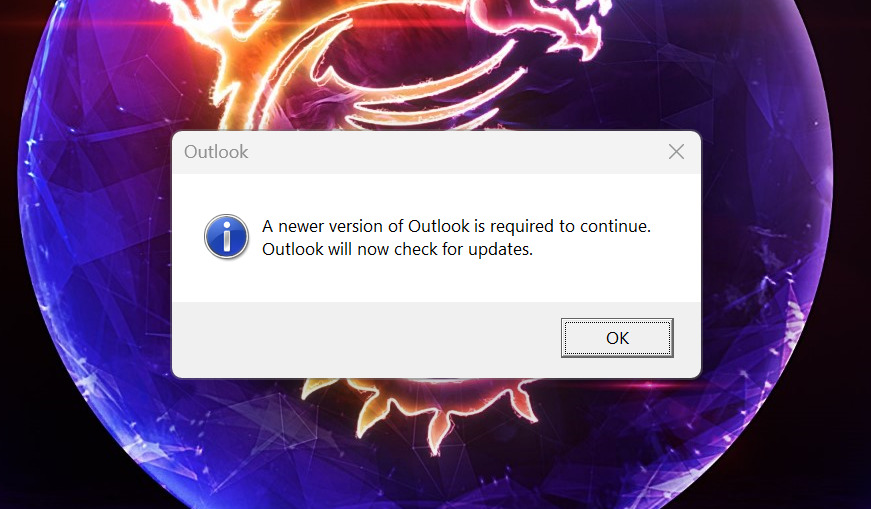
\includegraphics[width=0.5\linewidth]{visuals/outlook_requires_update.jpeg}
    \caption{Error Message after executing Forwarding Payload on MSI laptop}
    \label{fig:builtInTeensy}
    \cite{farhiMalboardNovelUser2019}
\end{figure}


Another big challenge with this payload is its UI focus. It requires a lot of settings menu navigation which is very time-sensitive. Short delays are detrimental here. Even for the MSI laptop which has the most compute of the tested devices, an especially long delay for opening Outlook and a delay of around 300ms between every navigation step is necessary to ensure that every TAB and ARROW input is correctly placed. \\
On the Microsoft Surface laptop, the attack worked as expected, which can be attributed to the fact that it was built while continuously being tested on this device. For none of the other test objects did the payload work out of the box, each would require updates, new logins or even lack the new Outlook completely. 

The conclusion for this payload is that it is not versatile and indeed requires a rather specific set of circumstances to work. Its UI focus makes this even harder since delays have to be high to accommodate the long loading times of an application like Outlook. If it works correctly, however, the payload can be very powerful and useful for gathering intelligence. 


\subsubsection{Disable Windows Event Logging}

GOAL: Disable Windows Event logging to hide possible traces another attack might leave. \\
PREREQUISITES: Windows 11

This payload has two versions; UI and CLI-based approaches, as discussed in chapter \ref{Implementation}. For the UI-based version, the usual problems occur; loading times, pop-up problems, and unforeseen reactions by the host. However, since this time the payload navigates through Windows Settings panels and not Outlook, some more continuity and speed can be expected. There are no server calls to be made that influence loading times, instead the process should be more straightforward. 
The Command Line Version should be even more reliable. It contains fewer steps and therefore less margin for error. It is expected to run smoothly on all test subjects.

The first execution of the UI-based approach proved once again its flakiness; Disabling Widows event logging on the MSI laptop would have also stopped another process, which caused the pop-up to confirm the action. This was not foreseen by the payload and therefore interrupted the process to the point where it exited the settings panel by selecting ``cancel'' instead of ``apply'' thereby ruining its progress. A second execution successfully stopped Windows event logging, since the pop-up did not appear again. However, it failed to close the settings window, leaving a trail of the attack. The navigation on the other side, was more reliable than what could be observed with the email forwarding payload which is as expected. \\
What was unexpected were language setting problems. When testing the payload on the TODO gaming desktop, it ran into problems because the search did not yield Windows event logging, but instead ``Windows Defender Advanced''. The payload would have to be adjusted to find the German ``Windows-Ereignisprotokoll''. After this adjustment, however, the next problem occurred; since the User did not have administrator rights, the settings options were greyed out and the payload had no chance of succeeding. \\
The payload worked well on the Surface Laptop, as expected since it was developed on it.

The CLI approach yielded much better results succeeding on the first try on the MSI laptop. As well as working on the custom-built gaming computer after adjusting the payload to enter the administrator password. As expected it also worked well on the Microsoft Surface Laptop. This result solidifies the superiority of a command line approach as opposed to navigating user interfaces. 


Conclusively it can be said that this payload works very well when applying the CLI approach. The UI version can work as well but requires a lot of fine-tuning, administrator access, and English as the system language. 



\subsubsection{Extract SAM hashes}

GOAL:\\ Extract SAM hashes from default storage on a device and send them to a command and control (C\&C) server.
PREREQUISITES: Windows 11 and a running C\&C server, in this case, Dropbox. Administrator rights are required

Since this script is working with default Windows settings, there are not a lot of challenges to be expected. On the MSI laptop, it worked flawlessly after some adjustments on the delays for opening the terminal. Since administrator access is not given on the custom gaming computer, the payload had to be adjusted to include the administrator password. With this adjustment, it was able to run successfully. The best results were again on the Windows Surface Laptop, where it executed flawlessly. 


\subsubsection{Extract Private Key Files}

GOAL: Find files that have extensions commonly used for private key files and send them to a C\&C server. \\
PREREQUISITES: Knowledge about the file system

This payload needs an entry point, some path to a local folder from which it can search through the files. If this is chosen too generally there may be permission issues. The entry point also heavily influences the time this payload takes to execute since it determines how many files the loop has to go through. The longer the script takes to execute, the easier it is to spot. \\
Since this payload does not require admin privileges one challenging step of opening an admin terminal is eliminated. One unexpected factor for errors is the validity length of the Dropbox access token. It expires within 4 hours. This means that in between saving the payload to the cable and the execution not more than those few hours may elapse. It was not a problem to adjust the payload for manual testing, however, this eliminates a C\&C server like Dropbox for boot scripts with unknown execution times. \\

The payload generally worked well on the Microsoft Surface laptop; its file system is known and an adequate entry point could be chosen. The execution was a success on the MSI laptop and the custom desktop as well. These good results could be due to the fact that apart from starting PowerShell, there are no loading times that can throw off the execution of the payload. Even waiting for the loop to end was not a problem; although delays were not adjusted to the expected search time, PowerShell still recognized and executed the command after finishing the loop.



\subsubsection{Steal Web Session Cookies}

GOAL: Figure out the target's default browser, then steal the web session cookies. \\
PREREQUISITES: None

This payload is pretty straightforward. Nevertheless, challenges for its flexibility arise. Executing the payload on the Microsoft Surface device went expectedly well, however, upon execution on the MSI laptop an error message occurred. Although the default browser on both of these devices is set to Firefox, their versions differ. While the Surface laptop had a slightly older version ( 129.0.1) the MSI laptop ran on the newest release, 129.0.2. This is reflected in the path to their cookies file. The .2 version stores the cookies at ``\textbackslash Mozilla\textbackslash Firefox\textbackslash \textbackslash Profiles\textbackslash dpsymep9.default-release\textbackslash cookies.sqlite''  while .1 stores them at ``Mozilla\textbackslash Firefox\textbackslash Profiles\textbackslash umva4gfp.default-release\textbackslash cookies.sqlite'' . This unexpected little, but crucial detail, derailed the execution of the script on the MSI laptop. The Chrome cookies path seems to be more robust; it worked without adjustments after changing the default for the MSI laptop to Chrome. The same problem occurred with the execution on the custom-built computer; it is running Firefox version wkbzpjnx. A more flexible version of this payload would check for versions and insert them as variables in the string, similar to how it does it with the Username environment variable. 

Apart from the version issues this payload performed well and as expected. 


\subsubsection{Iteratively End Processes}



GOAL: Certain processes should be ended as soon as they are detected as running. In whitelist mode, all programs except a few should be ended when they are detected as running.\\
PREREQUISITES: Windows 11, no admin rights required


This payload worked surprisingly well on the very first try. The MSI laptop posed no problem at all, not even delay adjustments had to be made. It worked as expected, terminating processes from the whitelist. As expected, the payload executed well on the Microsoft Surface, and on the desktop as well. \\
The only aspect that posed some problems was the minimizing of the window after the execution of the payload. It seemed that the ``ALT SPACE'' keypresses were not registered by the device and were not acted upon. On every device, the window was simply left open creating an obvious drawback for this payload; it is easy to spot and stop manually. 

\subsubsection{Schedule Processes}

GOAL: Schedule a job on the target device to execute a chosen script at a chosen time. \\
PREREQUISITES: Windows, administrator privileges

In order to test this payload, I set the script of the job to be \verb|Get-Process|. Execution on the MSI laptop worked well. However, it is important to note, that executing the payload twice back to back will generate an error because the process ``ProcessJob'' is already registered. To confirm the registration of the job, the Windows Scheduler Application can be used. The process should be listed under task scheduler library -> Microsoft -> Windows -> PowerShell -> ScheduledJobs. \\
Execution on the Surface Laptop went without issues as well. A challenge for the desktop is that the payload requires admin privileges. After adjusting the payload to enter the admin password, the payload is executed without any issues. 

\begin{figure}[H]
    \centering
    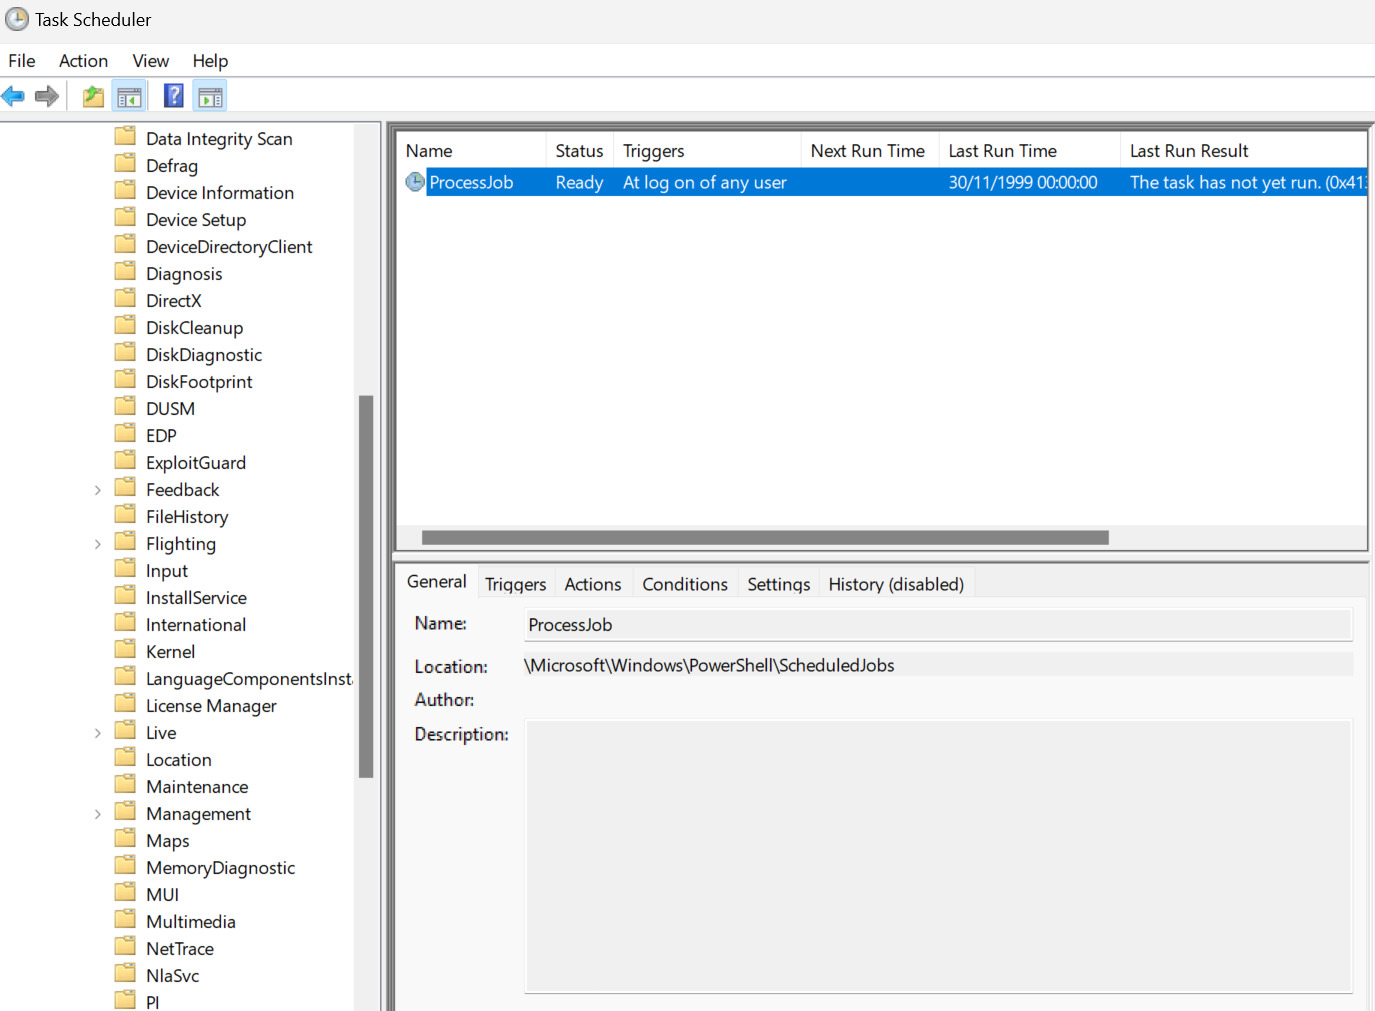
\includegraphics[width=0.5\linewidth]{visuals/task_scheduler_MSI.jpeg}
    \caption{Task Scheduler on the MSI laptop after successful registration of the Job}
    \label{fig:TaskScheduler}
\end{figure}



\subsection{Conclusion Attack Evaluation}


\section{Defence Evaluation} \label{defence evaluation}


This section will evaluate the performance of the defence script. To illustrate the progress a payload makes before it is interrupted, this thesis proposes a new metric. It measures the success of the payload in executed keystrokes divided by the total keystrokes in the payload. Executed keystrokes include commands such as \verb|ENTER| or \verb|LEFTARROW|and commands such as \verb|GUI R| are counted as two keystrokes. Variable length inputs, such as the email address to forward to in ''Register Email Forwarding`` are not considered in the total keystrokes of a payload. The benefit of this metric is that it represents how close the payload got to executing completely and achieving the attacker's goal. Its biggest disadvantage is that it does not reflect the actual success of the payload, since it does not take into account whether the input happened at the correct place and time. For example, a payload could execute 100\% of its keystrokes, but if there was an error along the way the payload likely still failed. This is why the metric is complemented by a qualitative description of the result to describe the end state of the payload. In the case of 100\% execution with an error along the way, it would state that the PowerShell script experienced an error and did not execute successfully. 

A spam payload is introduced to get a baseline for the performance of the executions without any delays or unknown factors. It's a simple script that does nothing besides set the keyboard language and input a sequence of ``qwertz'' until it reaches 2’400 characters. Listing \ref{lst:spam_payload} shows an excerpt of this script. 


\begin{lstlisting}[caption={Excerpt: write a string of length 2'400 without delays},label=lst:spam_payload, captionpos=b]
DUCKY_LANG DE_CH
STRING qwertzqwertzqwertzqwertzqwer
\end{lstlisting}

The execution of this script against all the following versions of the defence script provides a comparative value for the other payloads.
As a baseline, the speed of input for O.MG cables is determined. Theoretically, the O.MG cables are advertised to have input speeds of 120 keys/sec for the basic version and 890 keys/sec for elite. This evaluation will focus on 120 k/s to cover all versions of the O.MG cable. Considering this speed and the length of the payload, it should take 2'400 / 60 = 20 seconds to fully execute the script. To test this, the payload is executed and its frames examined. The epoch time stamp of the first HID packet subtracted from the timestamp of the last HID packet equals the elapsed time. These timestamps are displayed in Wireshark and can therefore easily be accessed. Testing results in execution times between 19.45 and 20.5 seconds, which is exactly the expected range. \\
Typing time can be categorized into two components: the interval between keystrokes and the duration each key is pressed. In terms of USB packets, this means a packet with HID data is first sent to the host to indicate a key press. After the duration of the key press, a second packet with HID data set to zeros is sent to indicate the key release. Holding a keypress delays this release package, signalling to the host to interpret the signal as autorepeat. This release frame can also be replaced by another key press package, to communicate to the host that a different key is pressed now. Understanding this mechanism is vital for comprehending the total number of keypresses a host registers when using the O.MG keyboard. A normal human user always has a delay between releasing a key and pressing another. The computer chip inside the cable does not have that constraint, it can simply send a new keypress signal to indicate a new keypress. This means that for O.MG input, the string ``aaa'' is actually 6 packets long, while ``abc'' has a length of 4. 

a b c [release] = 4
a [release] a [release] a [release] = 6

Therefore it is important to use a spam payload that does not consist solely of one character, it would increase the number of packets sent to the host in a way that is not representative of a usual payload.


[TODO explain the heuristic eval approach and devices]

In the following subsections, the two components of the defence script are evaluated separately: first, the enumeration pattern detection, and then the two options for the rate limiter.



\subsection{Enumeration Pattern Detection}

This subsection will describe a series of experiments to evaluate the enumeration pattern analysis (EPA). For these experiments, every payload is ran against the defence script with the rate limiter disabled, as shown in Listing \ref{lst:start_script_dr}, leaving only the enumeration analysis to detect O.MG devices.

\begin{lstlisting}[caption={start defence Script with Rate Limiter disabled},label={lst:start_script_dr}, captionpos=b]
 py .\omg_detection.py "USBDeview file path" -dr
\end{lstlisting}

Since this detection mechanism is based on a feature of the O.MG cable itself as opposed to any of the characteristics of a payload, it is expected to not have any differences in performance between the payloads. \\
The following list explains the qualitative and quantitative progress every payload made.

\begin{itemize}
    \item  \emph{spam}: 42 characters were written by the payload before it stopped. | 42/2400
    \item  \emph{Register Email Forwarding:} The interruption happened after the Windows Search Menu was opened, without the payload being able to search for anything  |  1/70 
    \item  \emph{Disable Windows Event Logging CLI:}  Execution stopped at the pop-up to confirm user privileges. | 3/95
    \item  \emph{Disable Windows Event Logging UI:} The attack reached the Windows run window without typing anything in | 2/47
    \item  \emph{Extract Hashes:}  The payload progressed until the pop-up window confirming user privileges. | 3/583
    \item  \emph{Extract Private Key Files:}  | Although no input was made, the payload did manage to open PowerShell. 164/1024
    \item  \emph{Steal Websession Cookies:} The attack was stopped right after opening PowerShell. | 16/1157
    \item  \emph{Iteratively End Processes:} The cable was disconnected after opening PowerShell. | 16/386
    \item  \emph{Schedule Processes:} The disconnect happened during the User Account Control popup to confirm admin rights. | 3/209
\end{itemize}

\begin{table}[h]
\centering
\begin{tabular}{|c|c|}
\hline
Name & EPA  \\
\hline
spam & 42/2400 \\
\hline
Register Email Forwarding & 1/70  \\
\hline
Disable Windows Event Logging CLI &  3/95 \\
\hline
Disable Windows Event Logging UI & 2/47 \\
\hline
Extract Hashes & 3/583  \\
\hline
Extract Private Key Files & 16/1024 \\
\hline
Steal Websession Cookies & 16/1157 \\
\hline
Iteratively End Processes & 16/386 \\
\hline
Schedule Processes & 3/209 \\
\hline
\end{tabular}
\caption{Table of executions rates for EPA}
\label{table:EPA_results}
\end{table}

Every execution was interrupted successfully before it could make any impact, often even before any of its intentions were clear. The effect of delays becomes obvious when comparing scripts that require admin rights with those that don't. That first group had many delays at the start of the script when opening menus and waiting for pop-ups. This gives the script a lot of time to react and disconnect the cable, hence the very low execution rates. The other group, on the other hand, uses the widows run menu to open PowerShell or Windows Services which is more input-heavy compared to the navigation of the first group. Start-heavy payloads are therefore able to input more keystrokes before the disconnect. In either case, the defence is a success, it detects the attack in 100\% of cases before anything can be executed. \\
However, still, the execution rates are not zero and are proof of the latency of the defence script. As is further evident by the result of the spam payload, which was able to input 42 keystrokes before it was interrupted.  Fortunately, such a script that spams input is not realistic as an attack scenario; in practice, every payload would have to waste time with delays, specifically somewhere at the start. 


\subsection{Rate Limiter}

This section will determine which values for the time window and interarrival time analysis respectively are best suited in defence against the newly formulated attacks.\\


\subsubsection{Interarrival Time Analysis}


This subsection discusses the interarrival time analysis, which tries to detect non-human input by its speed. Here, interarrival time is defined as the time between two key press signals. The time between key release and key press signal, which is often referred to in papers that analyze typing patterns, such as \cite{neunerUSBlockBlockingUSBBased2018}, is not applicable in this situation because of the way the O.MG cable generates its input. As discussed in the introduction to this chapter, Section \ref{defence evaluation}, the O.MG cable does not send key release signals when inputting a string, instead it simply sends the new keypress signal. Therefore this analysis cannot deal with durations between key release and new keypresses, they don't exist on many O.MG input sequences. Instead, this analysis focuses on the time between key press signals. \\
As established previously, the currently fastest human typing is at around 25 k/s, which comes out to approximately 40 milliseconds of interarrival time. The O.MG cable, at 120 k/s has a theoretical interarrival time of 8.3 milliseconds. 

To test these assumptions the script can be run with the command shown in Listing \ref{lst:start_script_ita_0.008,4}


\begin{lstlisting}[caption={start defence Script with ITA (0.008,4)},label={lst:start_script_ita_0.008,4}, captionpos=b]
 py .\omg_detection.py "USBDeview file path" -de --i "(0.008,4)"
\end{lstlisting}

The difficulty in finding a good configuration for the rate limiter lies therein, that an attack should always be registered as fast as possible (100\% true positives with 0\% false negatives) while keeping the alarms for human input as small as possible (0\% false positives).
This is a tradeoff, false positives will always be possible because the input speeds of a O.MG cable can easily be simulated by spamming a keyboard. As soon as multiple keys are pressed at the same time, the interarrival time between them is zero, triggering the rate limiter. This does not affect keys that are designed to compound, such as shift, control or alt, but pressing multiple character or number keys simultaneously will have that effect. This type of input is usually uncommon in real life, but can very easily happen by accident. \\
Nevertheless, the (0.008,4) configuration is not triggered by normal human input. It does not trigger for normal input speeds up to 90 wpm, and this subsection was written without any false positives. 

In the following, the performance of this configuration against the developed payloads is described quantitatively and qualitatively.

\begin{itemize}
    \item  \emph{spam}: 70 keystrokes were written by the payload before it stopped. | 70/2670
    \item  \emph{Register Email Forwarding:} The interruption happened after searching for Outlook(new) in the Windows Search Menu  | 14/70 
    \item  \emph{Disable Windows Event Logging CLI:}  The attack executed fully before the program attempted to disconnect it which failed because the cable had already disconnected autonomously | 95/95
    \item  \emph{Disable Windows Event Logging UI:} The script succeeded in opening Servies.msc but was stopped before navigating further. | 16/47
    \item  \emph{Extract Hashes:}  The payload progressed until the second line of the payload, without being able to exfiltrate anything. | 41/583
    \item  \emph{Extract Private Key Files:}  | Although no input was made, the payload did manage to open PowerShell. 16/1024
    \item  \emph{Steal Websession Cookies:} The attack was stopped right after opening PowerShell. | 16/1157
    \item  \emph{Iteratively End Processes:} Again the cable was disconnected after opening PowerShell. | 16/386
    \item  \emph{Schedule Processes:} The disconnect happened after the first line of the PowerShell script was executed, no harm was done at that point. | 39/209
\end{itemize}

In theory, this configuration (0.008 seconds averaged over 4 characters) should trigger a disconnect after the first 4 inputs; however, it takes until character 70 of the spam payload to disconnect. This is due to the defence script's latency. Since the input speed is so high, even a very small delay between the triggering keystrokes and the actual disconnect has a big effect.


Delays in the payload unexpectedly improved the performance of the rate limiter; after the first keystrokes to open a menu or application, the pauses allowed the program to react. Opening PowerShell as administrator requires a delay of at least 100ms after the first two input keystrokes to open the power user menu, increasing the average interarrival time significantly. This makes the start of the payload fly under the radar of the rate limiter. Only upon the start of the terminal input are the keystrokes continuous enough to reach the limit. This allows the payload to operate stealthily up to its PowerShell input. Additionally, it has a window of opportunity because the disconnect does not occur immediately after the first 4 continuous keystrokes, allowing it to use the delay to execute fully. This is what happened for ``Disable Windows Event Logging CLI''. It opened the PowerShell window without being detected and had enough time afterwards to execute the two lines of bash script that it needed to reach its goal. It was therefore able to run fully without being interrupted. When the defence script attempted to disconnect it, it had already deregistered itself. 

Payloads with many initial keystrokes were stopped the most quickly. They triggered the rate limiter by opening applications with the Windows Run Menu. Unlike opening applications with the Power User Menu, this approach requires the application's names to be typed out such that they trigger the rate limiter. The subsequent delays in the payload to allow the programs to start also afforded the defence script the time it needed to disconnect the devices.  

In conclusion, this configuration succeeds in detecting all the payloads, reacting faster with start-heavy payloads. Payloads with delays spacing out the input at the start have more success, even going as far as executing fully before being forcefully disconnected. An attempt to counteract this is shown in Listing  \ref{lst:start_script_ita_0.008,2}   

\begin{lstlisting}[caption={start defence Script with ITA (0.008,2)},label={lst:start_script_ita_0.008,2}, captionpos=b]
 py .\omg_detection.py "USBDeview file path" -de --i "(0.008,2)"
\end{lstlisting}

This payload is expected to recognize inputs faster, minimizing the delay, since it can react two keystrokes earlier than the previous configuration. 

This configuration is, however much less user-friendly. Since it averages over two keystrokes only, one particularly fast sequence of keystrokes can trigger the rate limiter, making it very prone to false positives. Even typing moderately fast at approximately 50 wpm triggers the rate limiter. Unlike the previous configuration, this does not allow comfortable typing speeds. Such a defence would be completely infeasible in practice, impractical defence systems are not supported by users, which is vital for their success. An average over three keystrokes might therefore be more useful and minimize false positives while also keeping the delay minimal. This configuration is shown in Listing  \ref{lst:start_script_ita_0.008,3}   
\begin{lstlisting}[caption={start defence Script with ITA (0.008,3)},label={lst:start_script_ita_0.008,3}, captionpos=b]
 py .\omg_detection.py "USBDeview file path" -de --i "(0.008,3)"
\end{lstlisting}

An average over three keys is much less susceptible to false positives and is not triggered by typing speeds around 80 to 90 wpm. It is therefore much more user-friendly. The following experiments evaluated whether it was faster at interrupting the payloads. 

\begin{itemize}
    \item  \emph{spam}: 80 keystrokes were written by the payload before it stopped. | 80/2670
    \item  \emph{Register Email Forwarding:} The interruption happened after searching for Outlook(new) in the Windows Search Menu  | 14/70 
    \item  \emph{Disable Windows Event Logging CLI:}  Execution stopped after the first line of the PowerShell script. | 41/95
    \item  \emph{Disable Windows Event Logging UI:} The script succeeded in opening Servies.msc but was stopped before navigating further. | 16/47
    \item  \emph{Extract Hashes:}  The payload progressed until the second line of the payload, without being able to exfiltrate anything. | 38/583
    \item  \emph{Extract Private Key Files:}  | Although no input was made, the payload did manage to open PowerShell. 16/1024
    \item  \emph{Steal Websession Cookies:} The attack was stopped right after opening PowerShell. | 16/1157
    \item  \emph{Iteratively End Processes:} Again the cable was disconnected after opening PowerShell. | 16/386
    \item  \emph{Schedule Processes:} The disconnect happened after the first line of the PowerShell script was executed, no harm was done at that point. | 39/209
\end{itemize}



The effects of decreasing the number of considered keystrokes are not particularly large. But can be observed in some instances. Table \ref{table:ITA_vs_ITA} compares the results for the two configurations. 

\begin{table}[h]
\centering
\begin{tabular}{|c|c|c|c|}
\hline
Name & ITA(0.008,4) & Comparison & ITA(0.008, 3) \\
\hline
spam & 70/2670 & < & 80/2670 \\
\hline
Register Email Forwarding & 14/70 & = &  14/70 \\
\hline
Disable Windows Event Logging CLI & 95/95 & > & 41/95 \\
\hline
Disable Windows Event Logging UI & 16/47 & = &  16/47 \\ 
\hline
Extract Hashes & 41/583 & > &  38/583 \\
\hline
Extract Private Key Files &  16/1024 & = &  16/1024 \\
\hline
Steal Websession Cookies &  16/1157 & = & 16/1157 \\
\hline
Iteratively End Processes & 16/386 & = & 16/386 \\
\hline
Schedule Processes & 39/209 & = & 39/209 \\
\hline
\end{tabular}
\caption{Table comparing the execution rates for ITA(0.008,4) and ITA(0.008,3)}
\label{table:ITA_vs_ITA}
\end{table}


Surprisingly the spam payload had even less success, although this result can be attributed to the testing approach rather than statistical significance. More importantly, the differences for most of the realistic payloads especially the start-heavy scripts such as ``Disable Windows Event Logging UI'' and ``Extract Private Key Files'' were non-existent. The interesting effect could be observed for end-heavy payloads that progressed further; specifically ``Disable Windows Event Logging CLI'' could no longer execute fully and was cut off after the first line. ``Extract hashes'', which has a similar structure, was also stopped earlier while the last end-heavy payload, ``Schedule Processes'' had the same result, possibly because the defence was able to use a delay in the PowerShell script to process the disconnect.  


Conclusively it can be said that an interarrival time of 0.008 seconds has a 100\% true positive rate to detect O.MG attacks. An average over 3 keystrokes supports it in minimizing false positives while keeping delays to a minimum.



\subsubsection{Time Window Analysis}


To get comparable results to ITA, TWA should be allowed to react after 3 keystrokes. Considering an input speed of 120 k/s, this results in a time window of 25 milliseconds or 0.025 seconds. What this configuration looks like for the defence script is shown in Listing \ref{lst:start_script_twa_0.025,3}.

\begin{lstlisting}[caption={start defence Script with TWA (0.025,3)},label={lst:start_script_twa_0.025,3}, captionpos=b]
 py .\omg_detection.py "USBDeview file path" -de --i "(0.025,3)"
\end{lstlisting}



This configuration is not triggered by human inputs of around 80 wpm. However, it also fails to detect the spam payload and thereby already fails with the very basic test. Most likely this is due to the delay in the defence script. Whenever a keystroke is registered, its timestamp is added to an array of recent timestamps. The script then scans that array for timestamps that are no longer in the considered time window, in this case, the present time minus 0.025 seconds. As soon as the delay between the arrival of the key press packet and its processing by the rate limiter takes longer than 25 milliseconds, that packet will immediately be removed from the timestamps array. Therefore that array will always be empty after it has been cleaned from keystrokes supposedly happening outside the time window and will never have a length of 3 or more. A longer time window is necessary to ensure the defence has a chance of detecting an O.MG cable.

For example, the time could be doubled as shown in Listing \ref{lst:start_script_twa_0.05,6}.

\begin{lstlisting}[caption={start defence Script with TWA (0.05,6)},label={lst:start_script_twa_0.05,6}, captionpos=b]
 py .\omg_detection.py "USBDeview file path" -de --i "(0.05,6)"
\end{lstlisting}

This configuration does also not trigger from human inputs of around 80 wpm. However, exactly as before, it will not be triggered by the spam payload and has therefore no chance of detecting any of the actual attacks.


A quick test of a (0.1,12) configuration shows that it too, will not recognize payloads reliably, it is therefore time to change the strategy.
Since the delay of the script seems to hinder it in recognizing keystrokes, adding that delay to the time window might soothe the problem. Listing \ref{lst:start_script_twa_0.125,3} shows the configuration for detecting 6 keystrokes within a time window of 72 milliseconds seconds plus 0.1 milliseconds of puffer to account for the script delay. 

\begin{lstlisting}[caption={start defence Script with TWA (0.125,3)},label={lst:start_script_twa_0.125,3}, captionpos=b]
 py .\omg_detection.py "USBDeview file path" -de --i "(0.125,3)"
\end{lstlisting}

This time, the rate limiter recognized and stopped the attack after 57 characters of the spam payload, a very good time. However, compromise on user input would be too high, this configuration has a high false positive rate. A compromise has to be made and a good candidate seems to be a (0.075,3) configuration. It could not be triggered by human typing of about 80wpm but detected spam input at 72 characters, a good start. This is the evaluation for Listing \ref{lst:start_script_twa_0.075,3}. 


\begin{lstlisting}[caption={start defence Script with TWA (0.075,3)},label={lst:start_script_twa_0.075,3}, captionpos=b]
 py .\omg_detection.py "USBDeview file path" -de --i "(0.075,3)"
\end{lstlisting}


\begin{itemize}
    \item  \emph{spam}: 72 characters were injected before the disconnect. | 72/2670
    \item  \emph{Register Email Forwarding:} The payload was interrupted after searching for Out-
look(new) in the Windows Search Menu | 14/7
    \item  \emph{Disable Windows Event Logging CLI:} Execution stopped after the first line of the
PowerShell script. | 41/95
    \item  \emph{Disable Windows Event Logging UI:} The script succeeded in opening Servies.msc
but was stopped before navigating further. | 16/47
    \item  \emph{Extract Hashes:}  One and a half lines of the PowerShell script could be typed out. | 38/728 
    \item  \emph{Extract Private Key Files:}  PowerShell was opened without any input. | 16/1024
    \item  \emph{Steal Websession Cookies:} Once again PowerShell was opened and did not receive any input. | 16/1157
    \item  \emph{Iteratively End Processes:} Just as previously, PowerShell was opened without input. | 16 /386
    \item  \emph{Schedule Processes:}  Progress was made until the second line of the PowerShell script where it was interrupted. | 54/209
\end{itemize}

These numbers are similar to the results from ITA, stopping start-heavy payloads the quickest, right after a long input and a delay to open PowerShell or Services.msc. Payloads that used the Power User Menu progressed further up to one or two lines of their PowerShell scripts. \\
This configuration achieved a true positives rate of 100\% with zero false negatives at input speeds of 80wpm of normal input. Considering the 25 k/s of maximum human input speed, a human would not be able to trigger this rate limit, since it takes 120 milliseconds at 25 k/s to type 3 keys. However, same as with ITA the limit can be exceeded by pressing multiple character and or number keys at a time. \\
The question arises whether results can still be improved upon; would a threshold of 2 characters within the time window interrupt payloads even quicker? Using the same ratio, this results in a configuration such as shown in Listing \ref{lst:start_script_twa_0.05,2}. 


\begin{lstlisting}[caption={start defence Script with TWA (0.05,2)},label={lst:start_script_twa_0.05,2}, captionpos=b]
 py .\omg_detection.py "USBDeview file path" -de --i "(0.05,2)"
\end{lstlisting}

\begin{itemize}
    \item  \emph{spam}:  | 70/2670
    \item  \emph{Register Email Forwarding:} Although Outlook(new) was searched for in Windows Search, it was not opened.  |63/70 
    \item  \emph{Disable Windows Event Logging CLI:} The payload was interrupted at the pop-up for confirming user privileges. | 3/95
    \item  \emph{Disable Windows Event Logging UI:} The script opened Windows Service settings without navigating further.  | 6/47
    \item  \emph{Extract Hashes:} It did not get further than the user Account Control pop-up. | 3/728 
    \item  \emph{Extract Private Key Files:} Powershell was opened without any input. | 16/1024
    \item  \emph{Steal Websession Cookies:} Again, PowerShell opened but did not receive input. | 16/1157
    \item  \emph{Iteratively End Processes:} One more time the interrupt happened after opening PowerShell.  | 16/386
    \item  \emph{Schedule Processes:}  The payload stopped once more at the pop-up. | 3/209
\end{itemize}

Next to a 100\% detection rate this configuration also performed very fast; stopping all end-heavy payloads already before they even opened PowerShell and interrupting all other payloads before they could input anything into their respective applications (PowerShell, services.msc, Outlook). \\
Interestingly this configuration is also more resistant to pressing multiple keypresses at once than ITA. Any number of keys can be pressed at once without setting off the rate limiter; it only activates when pressing multiple keys at the same time repeatedly. 
Further improving this configuration is not possible; decreasing the time window would only help against the delays if the number of keystrokes could be decreased as well. That is, however, not possible. With only one keystroke necessary in a time window to trigger the rate limiter, the false positive rate would be at 100\%.

In conclusion, (0.05,2) seems to be the best arrangement for TWA, with a detection rate of 100\%, no false positives, and a response time that can no longer be improved upon.




\subsection{Conclusion Defence Evaluation}

Table \ref{table:comparatvie_table_defence_eval} summarizes the result for the different defence configurations. 


\begin{table}[h]
\centering
\begin{tabular}{|c|c|c|c|c|c|}
\hline
Name & EPA &  ITA(0.008,4) & ITA(0.008,3) & TWA(0.075,3) & TWA(0.05,2)\\
\hline
spam & 42/2400 & 70/2670 & 80/2670 & 72/2670 & 70/2670\\
\hline
Register Email Forwarding & 1/70 & 14/70 & 14/70 & 14/7 & 63/70\\
\hline
DWEL CLI & 3/95 & 95/95 & 41/95 & 41/95 & 3/95\\
\hline
DWEL UI & 2/47 & 16/47 & 16/47 & 16/47 & 6/47 \\
\hline
Extract Hashes & 3/583 & 41/583  & 38/583 & 38/728 & 3/728\\
\hline
Extract Private Key Files & 16/1024 & 16/1024 & 16/1024 & 16/1024 & 16/1024 \\
\hline
Steal Websession Cookies & 16/1157 & 16/1157 & 16/1157 & 16/1157 & 16/1157\\
\hline
Iteratively End Processes & 16/386 & 16/386  & 16/386 & 16 /386 & 16/386\\
\hline
Schedule Processes & 3/209 & 39/209  & 39/209 & 54/209 & 3/209 \\
\hline
\end{tabular}
\caption{Comparative table of execution rates for EPA, TWA and ITA}
\label{table:comparatvie_table_defence_eval}
\end{table}


The fastest results are reached with enumeration analysis, followed by TWA(0.05,2) and a very close call between TWA(0.075,3) and ITA(0.008,3). For every defence option, a 100\% detection rate could be achieved, mostly while preventing the payload from executing and causing harm. The only instance in which a payload was able to reach (part of) its goal was ``Disable Windows Event Logging'' with ITA. Since EPA is triggered first before any keystrokes are injected, it can react fastest, while TWA(0.05,2) has the advantage over the other configurations in that it only has to wait for two keystrokes instead of three. \\
While these results are promising, it has to be kept in mind that the rate-limiting options are dependent on a specific type of input. Payloads that space said input in the right way, can circumvent the detection. The O.MG cable, for example, has a configuration option ``DEFAULT\_CHAR\_DELAY'' that can be set to add a delay after every string character. This way, the rate limiters can be tricked; more spaced input decreases the input speed and therein tricks the rate limiter into a false negative. [TODO: add a demonstration]. \\
In situations like these, ETA is essential; it cannot be tricked. The bm attributes of an O.MG cable cannot be set by a user themselves, not even if they write their own firmware, as confirmed by developers of Mischief Gadgets. It is not guaranteed, however, that this enumeration pattern is present in every BadUSB or will always exist on O.MG devices. A combination of different approaches is therefore recommended to ensure as many attacks as possible are detected and prevented from causing harm. 

